  \documentclass[linenumbers,twocolumn]{aastex631}

\usepackage{longtable}
\usepackage[flushleft]{threeparttable}
\usepackage{tabularx}
\usepackage{multirow}
\usepackage{graphicx}
\usepackage{amsmath,amssymb}
\usepackage{color}
\usepackage{units}
\usepackage{epstopdf}
\usepackage{hyperref}
\usepackage{multirow}
\usepackage{url}
\usepackage{subfigure}
\usepackage{rotating}
\usepackage{enumitem}\setlist[description]{font=\textendash\enskip\scshape\bfseries}
% \usepackage{lineno}

\usepackage[colorinlistoftodos]{todonotes}

% \linenumbers

%\usepackage[doublespacing]{setspace}

\newcommand{\braket}[2]{\left\langle#1\, |\,#2\,\right\rangle}  %  < #1 | #2 >
\newcommand{\expec}[1]{\langle#1\rangle}  %  < #1 >
\newcommand{\drm}{{\rm d}}
\newcommand{\irm}{{\rm i}}
\newcommand{\beq}{\begin{equation}}
\newcommand{\eeq}{\end{equation}}
\newcommand{\bdm}{\begin{displaymath}}
\newcommand{\edm}{\end{displaymath}}
\newcommand{\T}[1]{\tilde{#1}}
\newcommand{\wT}[1]{\widetilde{#1}}
\newcommand{\Cdot}{\!\cdot\!}
\newcommand{\SNR}{\textnormal{SNR}}
\newcommand{\rednote}[1]{{\color{red} (#1)}}
\definecolor{Gray}{gray}{0.9}
\definecolor{orange}{rgb}{0.9,0.5,0}
\newcommand{\td}[1]{{\textcolor{orange}{\texttt{TD: #1}} }}
\newcommand{\zd}[1]{{\textcolor{purple}{\texttt{ZD: #1}}}}
\newcommand{\muj}[1]{{\textcolor{red}{\texttt{MU: #1}} }}
\newcommand{\sa}[1]{{\textcolor{blue}{\texttt{SA: #1}}}}
\newcommand{\ztfrest}{\text{ZTFReST }}
\newcommand{\ttt}[1]{\texttt{#1}}
\newcommand{\jp}[1]{{\textcolor{blue}{#1}}}

\newcommand{\nmma}{\text{NMMA }}

\newcommand{\ztfink}[1]{ZTF-Fink}
\newcommand{\fink}{{\sc Fink}}

% Load results from results.tex so these can be updated automatically
% This file was automatically generated; edits will be overwritten!
\newcommand{\boomthroughputfactor}{6}
\newcommand{\kakfaingestratembps}{XXXXX}
\newcommand{\kakfaingestfactor}{XXXXX}


%\graphicspath{{./plots/}}

\begin{document}

\title{\texttt{BOOM} and \texttt{Babamul}: a real-time, multi-survey, optical alert system broker operating at scale}

\author[0009-0003-6181-4526]{Theophile Jegou du Laz}
\affil{Division of Physics, Mathematics, and Astronomy, California Institute of Technology, Pasadena, CA 91125, USA}

\author[0000-0002-8262-2924]{Michael W. Coughlin}
\affil{School of Physics and Astronomy, University of Minnesota, Minneapolis, Minnesota 55455, USA}

\author[0000-0003-4039-6954]{Peter Bachant}
\affil{California Institute of Technology, Pasadena, CA 91125, USA}

\author{Jacob E. Simones}
\affil{School of Physics and Astronomy, University of Minnesota, Minneapolis, Minnesota 55455, USA}
\affil{Department of Physics, University of Minnesota-Duluth Duluth MN 55812 USA}

\author[0009-0008-3603-0013]{Thomas Culino}
\affil{Division of Physics, Mathematics, and Astronomy, California Institute of Technology, Pasadena, CA 91125, USA}

\author[0009-0009-7000-8343]{Antoine Le Calloch}
\affiliation{School of Physics and Astronomy, University of Minnesota, Minneapolis, Minnesota 55455, USA}

\author[0000-0003-1314-4241]{Sushant Sharma Chaudhary}
\affil{School of Physics and Astronomy, University of Minnesota, Minneapolis, Minnesota 55455, USA}


% Abstract of the paper
\begin{abstract}
With the arrival of ever higher throughput wide-field surveys and a multitude of multi-messenger and multi-wavelength instruments to complement them, software capable of harnessing these associated data streams is urgently required. To meet these needs, a number of community supported \emph{alert brokers} have been built, currently focused on processing of Zwicky Transient Facility (ZTF; $\sim 10^5$--$10^6$ alerts per night) with an eye towards Vera C. Rubin Observatory's Legacy Survey of Space and Time (LSST; $\sim 2 \times 10^7$ alerts per night). Building upon the legacy of a successful system that ran in production for ZTF for the first seven years of its operation, we introduce \texttt{BOOM} (Burst \& Outburst Observations Monitor), an analysis framework focused on real-time, joint brokering of these alert streams.
Harnessing the performance of a \texttt{Rust}-based software stack relying on a non-relational (NoSQL) \texttt{MongoDB} database combined with a \texttt{Redis}/\texttt{Valkey} in-memory processing queue and a \texttt{Kafka} cluster for message sharing, we demonstrate feature parity with the existing ZTF system with a throughput $\sim \boomthroughputfactor \times$ higher.
We describe the workflow that enables the real-time processing, as well as results with custom filters we have built to demonstrate the system's capabilities.
We further outline the development plan for \texttt{BABAMUL}, the public version of \texttt{BOOM} processing LSST alerts.
Finally, we outline the development plans for \texttt{BOOM} as we begin the LSST era.
\end{abstract}

%%%%%%%%%%%%%%%%%%%%%%%%%%%%%%%%%%%%%%%%%%%%%%%%%%

\listoftodos

%%%%%%%%%%%%%%%%% BODY OF PAPER %%%%%%%%%%%%%%%%%%

\section{Introduction}

Modern optical surveys now scan the entire sky daily, reaching depths that allow detection of both distant, bright objects and nearby, faint ones. This capability enables the discovery of rare phenomena, a census of the variable sky, and tests of fundamental physics at energy scales far beyond those of terrestrial accelerators. However, fully exploiting these opportunities is currently constrained as much by software and data processing methods as by available instrumentation.
The upcoming Vera C. Rubin Observatory's Legacy Survey of Space and Time (LSST) exemplifies the scale of future transient discovery \citep{Ivezic2019}. LSST will scan large swaths of the sky to unprecedented depths. Each potential discovery will be immediately broadcast as an alert, not directly to the entire community but to a set of pre-selected alert brokers, tasked with redistributing the data stream to the wider community, while providing easy-to-use tools to search for and visualize candidates of specific astronomical objects.
For comparison, the Zwicky Transient Facility (ZTF) \citep{Bellm:19:ZTFScheduler,Graham2018,DeSm2018,Masci2019}, the current survey that the community most commonly uses for transient follow-up, produces $\sim 10^5$--$10^6$ alerts per night, while LSST will be more than an order of magnitude larger ($\sim 10^7$).

Real-time processing and rapid follow-up of this alert stream is critical for many science cases, with brokering software needing to keep up with the rate of alerts while maintaining or increasing the number of features it aims to offer to the end user. The alerts emitted by these large surveys include a variety of transient phenomena, including, among many other science cases,
\begin{itemize}
\item Very young Type Ia supernovae (SN\,Ia) with either an early ``flash'' or ``bump'' in their light curves well before the epoch of maximum light (e.g., iPTF14atg; \cite{cao_strong_2015}, SN2017cbv; \cite{Hosseinzadeh_2017} and SN2019yvq; \cite{Miller_2020})
\item Luminous fast blue optical transients (LFBOTs) \cite{PrMa2018,Perley2019,HoGo2019,HoPe2020,Perley_2021}, with optical and (sometimes) copious X-ray emission evolving on short timescales
\item $\gamma$-ray burst afterglows \cite{NyFr2009,GeMe2012} from either collapsars or neutron star mergers
\item Kilonovae associated with binary neutron star mergers \citep{AbEA2017b} such as AT2017gfo \citep{CoFo2017,SmCh2017,AbEA2017f}
\item Jetted tidal disruption events whose accretion leads to the launch of a relativistic jet \citep{Bloom2011Sci,Andreoni_2022}
\end{itemize}
These young and/or fast transient science cases are bolstered by the rise of instruments in other messengers, e.g., Advanced LIGO \citep{aLIGO} and Advanced Virgo \citep{adVirgo} for gravitational waves, e.g., IceCube \citep{AaAc2017} for neutrinos, or other wavelengths,  the {\it Neil Gehrels Swift Observatory} mission \citep{GeCh2004}, Fermi's Gamma-ray Burst Monitor (Fermi-GBM) \citep{MeLi2009}, the Space-based multi-band astronomical Variable Objects Monitor (SVOM), and Einstein Probe \citep{Yuan_2022} for $\gamma$-rays and X-rays.

There is a large software ecosystem enabling time-domain astronomy.
For example, the General Coordinates Network (GCN; \citealt{SiRa2023}) and the Scalable Cyberinfrastructure to support Multi-Messenger Astrophysics\footnote{\url{https://scimma.org/}} (SCiMMA) project are platforms where multi-messenger instruments share real-time alerts with the community that can then be either followed-up directly or cross-matched with alert streams.
Depending on the type of transient, it is common for identified objects to be shared with the community on the Transient Name Server\footnote{\url{https://www.wis-tns.org/}} (TNS) or the Minor Planet Center\footnote{\url{https://minorplanetcenter.net/}} (MPC).
These streams are ingested by Target and Observation Managers (TOM), otherwise known as ``marshals,'' which enable coordinated follow-up efforts; examples include \texttt{YSE-PZ} \citep{CoJo2023}, TOM Toolkit \citep{StBo2018}, and \texttt{SkyPortal} \citep{WaCr2019,Coughlin_2023}.

Feeding these marshals are the ``enriched'' alert streams from the brokers, including, among others, ALeRCE \citep{FoCa2021}, AMPEL \citep{Nordin:2019kxt}, ANTARES \citep{MaSt2021}, Fink \citep{MoPe2020}, Lasair \citep{SmWi2019}, Pitt-Google, and \texttt{BABAMUL} (the plans for which we will discuss further below). These brokers filter the optical alert streams to identify targets of interest. For surveys like ZTF and LSST, alerts are produced when a significant ($< 5 \sigma$) residual flux is detected from a point source in a subtracted image, and are distributed via Kafka\footnote{https://kafka.apache.org} in Apache avro format. While each survey provides a different set of data and, therefore, uses a different schema to serialize it, they all include key properties such as:
\begin{itemize}
\item Position and brightness of the current detection
\item Ancillary detection data and higher-level derived values, including real--bogus scores, which helps distinguish real transients from image artifacts.
\item The associated triplet of science, reference, and subtraction images
\item Time-series information about past alert-based detections, non-detections, and forced photometry
\item Higher-level metadata about a known astronomical object at the location of the detection (to within some positional uncertainty).
\end{itemize}

To identify the most interesting objects for particular science cases, brokers can cross-match alerts against static catalogs (e.g., Gaia DR3, \cite{Gaia2023}; PanSTARRs DR1, \cite{ChMa2016}; milliquas, \cite{Flesch_2023}; NED LVS, \cite{Cook_2023}) and look for specific properties using machine learning classification pipelines (e.g., AstroM3, \cite{rizhko2024astrom}; BTSbot, \cite{Rehemtulla+2024}; ACAI, \cite{duev2021phenomenologicalclassificationzwickytransient}; Maven, \cite{zhang2024mavenmultimodalfoundationmodel}). All brokers provide their own filtering system that makes use of the ``enriched'' alert data to identify objects of interest for specific science cases. Depending on the broker, the filters can be from a standard set defined based on community feedback or customized by the user directly. Also, they may run in real-time as alerts are coming in, or anytime after the alert data is processed to perform archival searches. So far, alert brokers have been providing these services predominantly for the ZTF alert stream. However, now that a number of surveys providing real-time alert streams will overlap in space and time, we -- as a community -- have an opportunity to enrich each survey with the data products from the others.

Specifically, to supplement the LSST alert stream, a variety of other optical systems such as the La Silla Schmidt Southern Survey (LS4; \citealt{miller2025lasillaschmidtsouthern}) and ZTF will be trailing the LSST footprint nightly. To maximize the science synergies enabled by these coordinated observations, brokers will need to perform joint filtering on these alert streams. This will be essential to, for example, readily identify fast transients within these streams, as the relatively slow cadence of LSST will otherwise make it difficult to identify such phenomena, and the limited depth from other optical surveys makes it difficult to precisely constrain their rate of evolution.

It is with these considerations in mind that we present \texttt{BOOM}, a broker that builds upon our experience with \texttt{Kowalski}\footnote{\url{https://github.com/skyportal/Kowalski}}, an open source, multi-survey data archive and alert broker \citep{DuMa2019} that the ZTF collaboration has run in production for the last seven years, with \texttt{SkyPortal} as its ``marshal``.
In this paper, we will describe several important developments and design choices made with \texttt{BOOM} that ready it for the upcoming LSST era.
Although this paper focuses mainly on the design and conceptual framework of \texttt{BOOM}, we encourage the interested reader to explore the repository alongside this text \footnote{https://github.com/boom-astro/boom}, and read its documentation.
As an example of important design choices, since multiple observatories will observe the LSST footprint concurrently, \texttt{BOOM} has as its top priority, the ability to jointly filter on multiple alert streams. A relatively unique capability in the broker community.
Furthermore, one of the main differences between \texttt{BOOM} and \texttt{Kowalski}---and most other alert brokers---was moving away from Python and instead writing the project in \texttt{Rust}, a compiled programming language with performance characteristics that make it much better suited to attaining a high throughput of alerts at scale. Processing additional alert streams in parallel increases the data volume by at least an order of magnitude, and jointly filtering on multiple streams requires even more computation, as every alert packet needs to be cross-matched with all other overlapping surveys' alert streams. While not relying on \texttt{Python} may have the downside of making contributions from astronomers - who typically write in Python - more challenging, our experience running \texttt{Kowalski} in production has shown us that requiring computer science knowledge to make use of an alert broker will significantly limit its use, and that regardless of complexity. Below, we will describe the filter building tool we have built to ameliorate this challenge, where the user is provided with a no-code alternative to write complex queries.

In this paper, we describe the components built within \texttt{BOOM}, focusing on design choices useful in preparation for LSST data scales.
We describe \texttt{BOOM}'s key features in Sec.~\ref{sec:pipeline}.
We demonstrate some of \texttt{BOOM}'s capabilities, including throughput measurements, in Sec.~\ref{sec:science}.
We describe the future of \texttt{BOOM} and how we envision its role in the community in Sec.~\ref{sec:conclusion}.

\section{\texttt{BOOM} Framework}
\label{sec:pipeline}

\begin{figure*}[t]
    \centering
    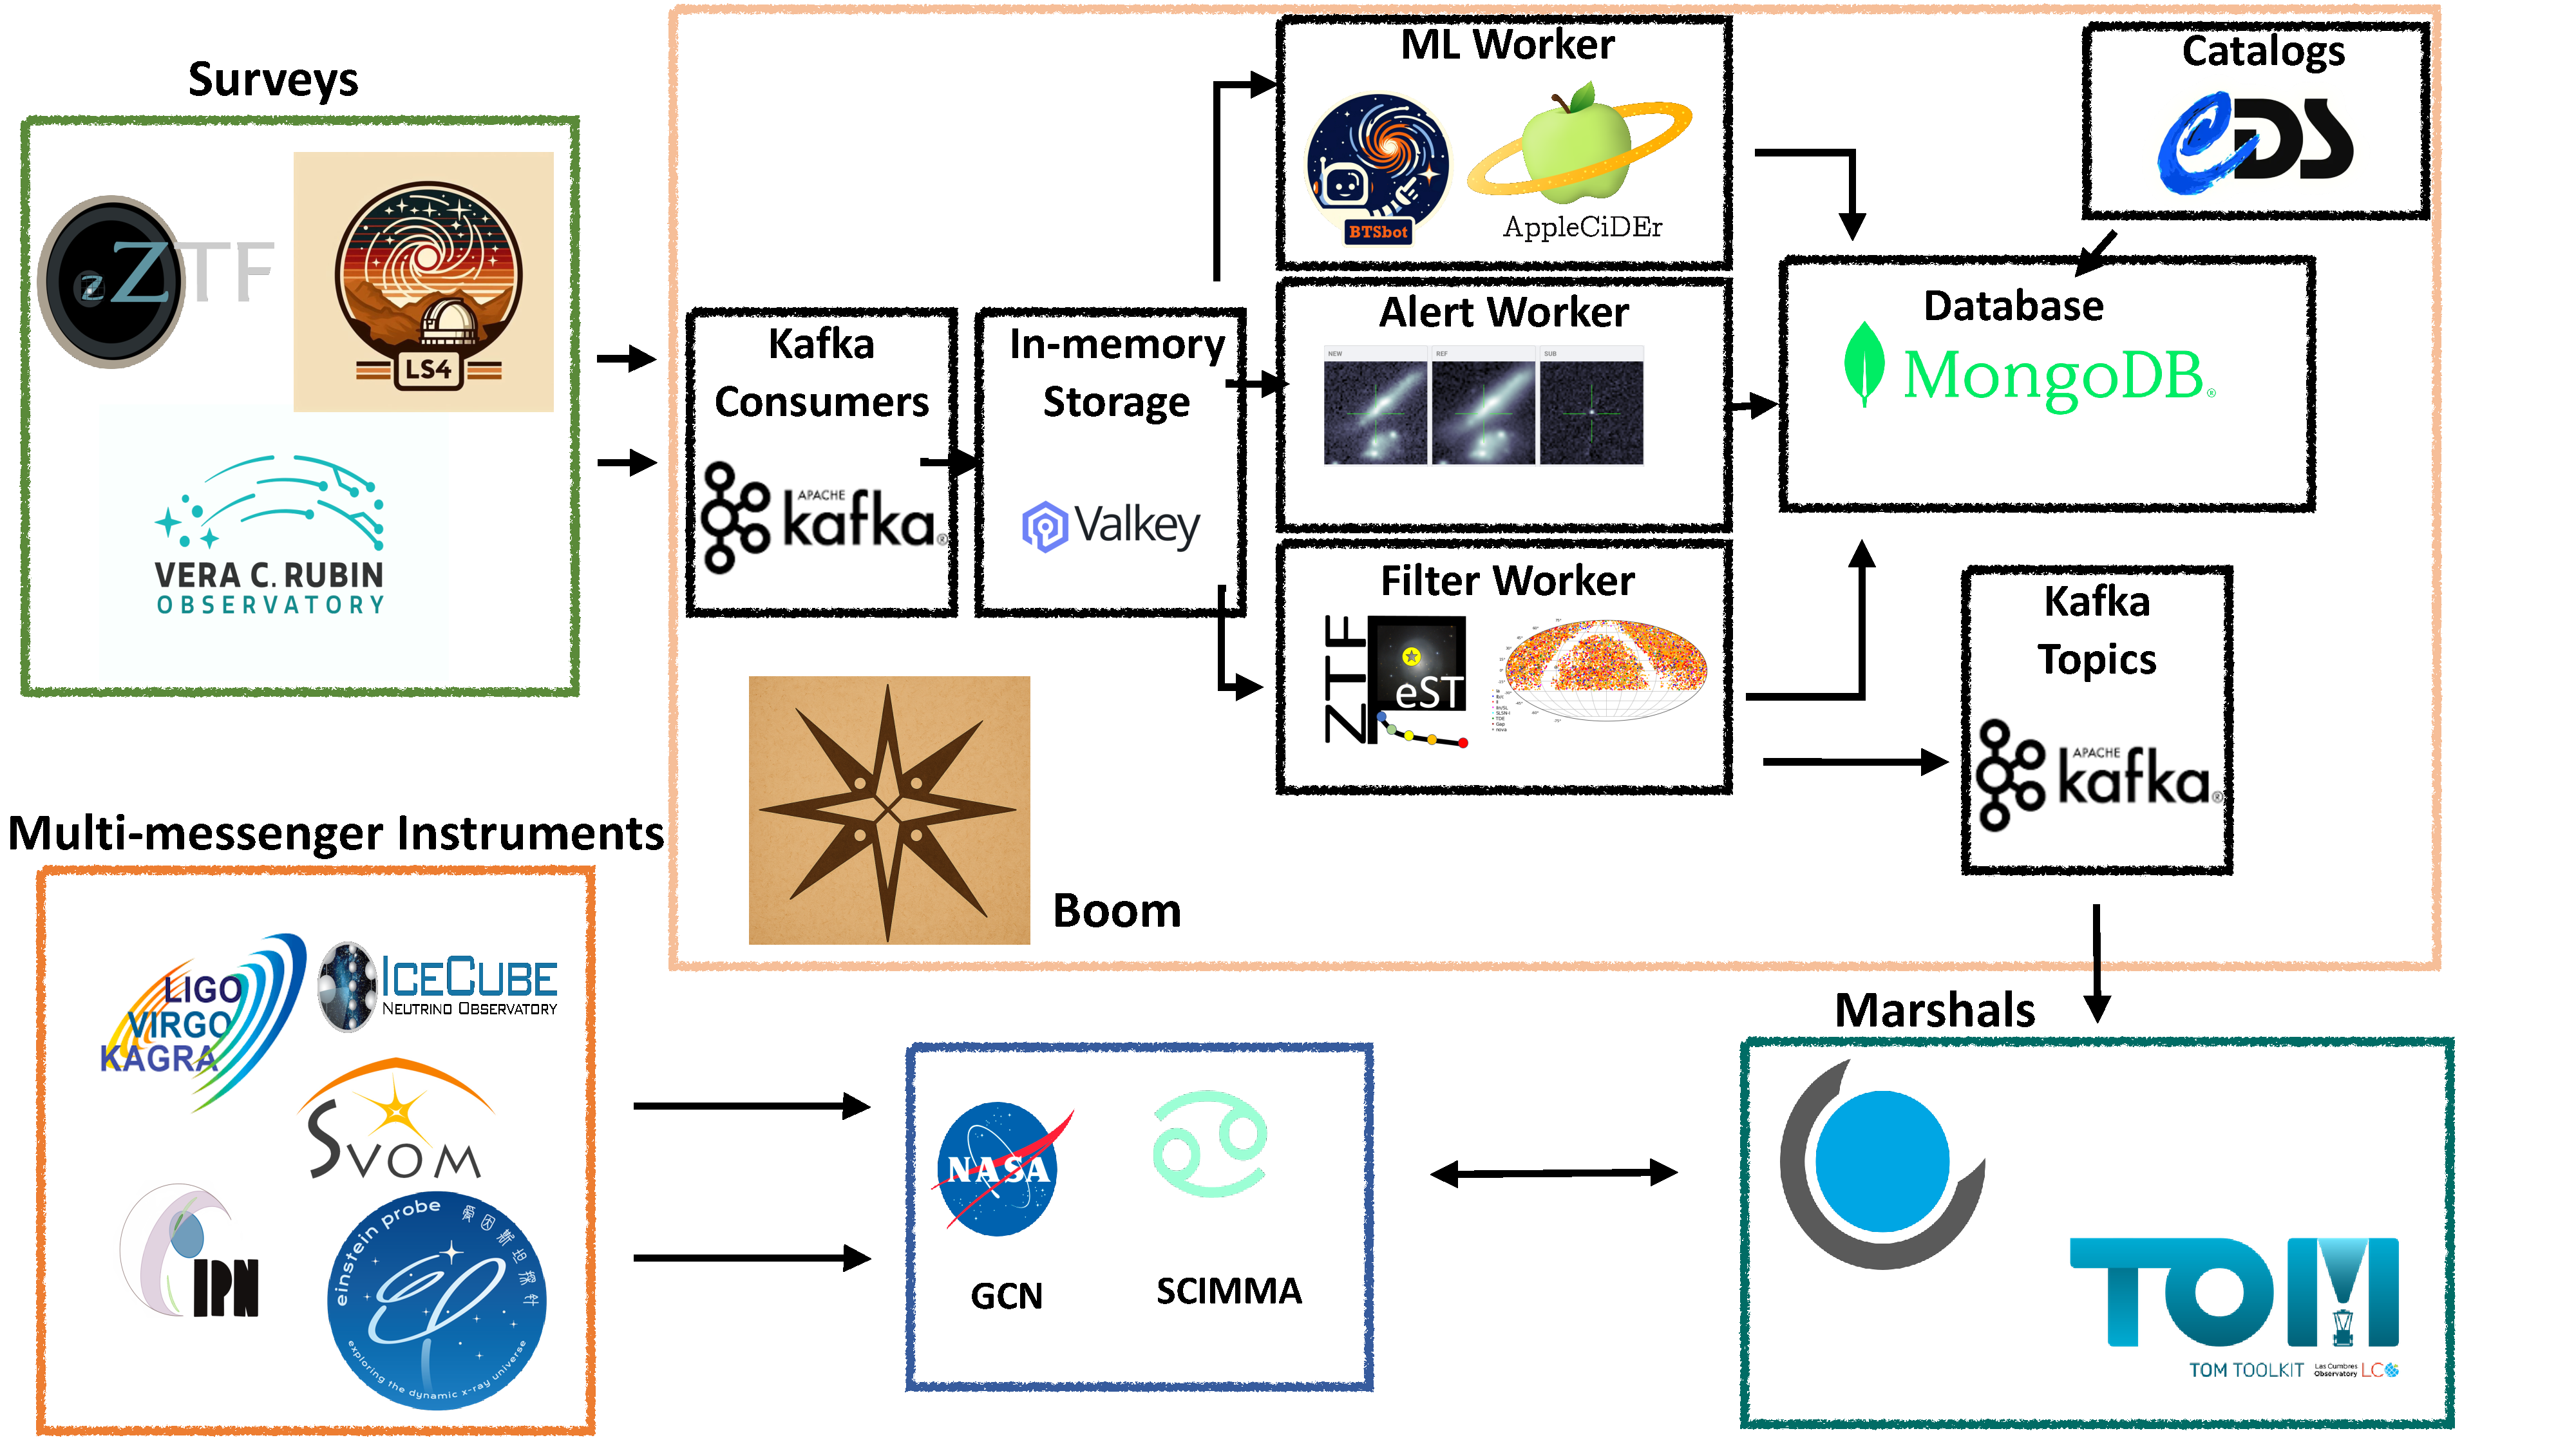
\includegraphics[width=6.5in]{figures/workflow.pdf}
    \caption{Flowchart for BOOM.}
    \label{fig:flowchart}
\end{figure*}

In this section, we present the key design features and implemented capabilities within \texttt{BOOM}.
\texttt{BOOM} is designed for full parallelization. The database and alert processors all scale horizontally, allowing additional workers to be added at any stage to accommodate changes in workload. Alerts can be processed in any order, meaning they do not need to follow a strict time sequence.
\texttt{BOOM} operates with workers, separating the machine learning, cross-matching, filtering, ingestion, etc. into different processes. Each of these workers are described herein.

\subsection{Input/Output through \texttt{Apache Kafka}}

\texttt{Apache Kafka} has become the gold standard for astronomical alert brokering due to its scalability, fault tolerance, and capacity to handle large data volumes for a wide variety of production-grade software, in academia and industry. Optical alerts from surveys like ZTF and LSST are transmitted as Avro packets\footnote{\url{https://avro.apache.org}} over \texttt{Kafka}, which means that the ability to feed from \texttt{Kafka} topics - which represent one data stream that a client can read from - is absolutely required by any alert brokering software. Its ecosystem of libraries available for all major programming languages makes it extremely easy for the client to develop pipelines around it. For these reasons, also adopting \texttt{Kafka} as our downstream data sharing system ensures compatibility with existing downstream services, which are designed to consume alerts from \texttt{Kafka} too. For each survey supported by our software, an associated \texttt{Kafka} consumer has been developed to feed from the \texttt{Avro}-formatted alerts. The consumers take advantage of \texttt{Kafka}'s partitioning feature (where one topic is broken down in N partitions that a client can read from independently, with multiple processes) to process any given survey's alert stream(s) in parallel, maximizing the input rate. \texttt{BOOM}'s output, as described in subsection X, is also serialized to \texttt{Avro} and produced to a \texttt{Kafka} cluster.

\subsection{Job scheduling with \texttt{Valkey}}

Whereas \texttt{Kafka} shines when it comes to reliable message sharing at scale across the Web, it is not the most performant solution for interprocess communication as its topics are stored on disk, which results in throughput limited by the host's I/O capabilities.
Instead, we opted for \texttt{Valkey}, a high-performance and open source in-memory datastore backed by the Linux Foundation.
\texttt{Valkey} can be used for a variety of workflows, including caching and message queues.
Unlike \texttt{Kafka}, all data stored by \texttt{Valkey} live in RAM, ensuring much higher throughput than physically possible with data stored on HDDs or SSDs. However, a `persistence` feature can also be enabled which lets \texttt{Valkey} periodically create backups on disk, so that its content can be restored in the event of a catastrophic failure. This process is performed asynchronously and did not show a noticeable impact on performance.
Once data is read from the various survey's \texttt{Kafka} topics, \texttt{BOOM}'s \texttt{Kafka} consumer stores alerts to be processed in \texttt{Valkey} lists; these are simple array data structures from which processes on the same machine or network can read from concurrently, one element at a time or in batches. When read from a list, messages are removed from it and one message can only be retrieved by one process. This is precisely what we need for \texttt{BOOM}, where alert processing is not performed by one but by many processes, to parallelize over the data streams. Message queues used by \texttt{BOOM}'s workers to communicate with each other only share a minimal amount of information: mostly pointers to database documents, and unique identifiers of alert packets. So, they do not have a significant memory impact. However, memory usage remains a concern when relying heavily on in-memory storage technologies for larger data products, such as the original \texttt{avro} alerts at the first stage of processing. With this in mind, \texttt{BOOM} sets limits on how many alert packets are stored in memory at once. Moreover, since \texttt{Valkey} is only used as a job queue, all lists are meant to be temporary and consumed as they are filled. As long as \texttt{BOOM} is configured to handle incoming alerts with little to no throttling, which means providing it with sufficient compute capabilities, these lists remain fairly empty and so does the overall memory usage.

\subsection{Spatial query-ready database with \texttt{MongoDB}}

\texttt{MongoDB} has proven to be a highly effective choice for alert brokering, as demonstrated by its successful implementation in \texttt{Kowalski}. Its cross-language support, flexibility, and powerful query language make it well-suited for building complex filtering pipelines for transient alerts. Namely, the \texttt{aggregation pipeline} feature has allowed us to define not only complex queries but also pipelines of queries with multiple stages, such as a cycle of filtering (\$match stage), computing (\$project, \$addField, \$lookup ... stages) steps, well-suited to implement astronomical alert filtering pipelines. \texttt{MongoDB} offers both performance and scalability, essential for handling large data volumes efficiently. It's built-in compression also simplifies data storing requirements. While \texttt{PostgreSQL} was a potential alternative, it would have required schema enforcement, which in turns requires database migrations whenever a new astronomical catalog is integrated for cross-matching or a new survey's support is added. Additionally, \texttt{MongoDB} natively supports \texttt{GeoJSON} indexes for fast spatial queries, such as cone-searches or nearest neighbour searches without any client-side implementation or extensions required, features that \texttt{PostgreSQL} does not implement natively. Just like \texttt{Kowalski}, \texttt{BOOM} relies very heavily on \texttt{MongoDB}'s native support for cone-searches between alert streams and archival/static catalogs, and on it's \texttt{aggregation pipeline} feature to design and execute complex user-defined filters. When it comes to our data model, alert packets are dividing into 3 distinct collections (\texttt{MongoDB's} equivalent of a table, as found in a relational context):
\begin{itemize}
    \item The \texttt{Alert} collection, containing an alert's \texttt{candidate}, metadata about the latest detection that resulted in the alert being sent. To which we later append time-dependent data products, such as machine learning scores and "pre-computed" features to facilitate the implementation of user-defined filter, as described in subsection Y. Entries of the collection are indexed on the alert's candidate ID (candid, a unique identifier provided by the associated survey), its object ID (objectId, an identifier for this astronomical object, most often purely position based: detections made at the position of a previous alert will be attributed the same objectId), and its position.
    \item The {Object} collection, containing lightcurve data products (concatenated from the time-limited lightcurves provided by each alert for the same object, as surveys provide only N days worth of past detections), and matches with other catalogs and surveys. For archival catalogs matches all the relevant metadata is stored in this collection, whereas for alert-based survey matches only the survey's objectIds are stored to enable lookups when user-defined filters are run. Entries of this collection are indexes on objectId, and on the object's position (taken from its first alert ingested by \texttt{BOOM}, which is subject to change as a flux-averaged centroid may be more adequate).
    \item The {Cutout} collection, simply containing the science, reference, and difference image cutouts from the alert packet. This collection is also indexed on the alert's candid, to enable quick lookups of alert images based on their identifier.
\end{itemize}

With this data model, the data-heavy images that cannot be queried like other data products would are stored on their own and can be optionally retrieved alongside alerts using lookups, and object-specific data products (i.e. positional based) such as cross-matches and lightcurves are stored in one place instead of on every alert (as served over \texttt{Kafka} by the various surveys), which would yield considerable duplication and increase data storage requirements.

\subsection{Parallelized and Distributed Alert Processing}

\texttt{BOOM} employs a different architectural approach than its predecessor \texttt{Kowalski}, using dedicated worker types for each processing stage rather than a single monolithic worker design. In \texttt{Kowalski}, alert processing was parallelized using a cluster of identical workers where each worker was responsible for the complete end-to-end processing of individual alert packets. This included performing database insertions and queries such as cross-matching with archival catalogs, running user-defined filters, inserting and updating alerts and objects, and running machine learning models. While this design simplified deployment and management, it suffered from significant inefficiencies that prevented it from scaling up sufficiently and efficiently.

The single worker-type approach creates several unavoidable bottlenecks. First, forcing a sequential processing of alerts one at a time prevents the system from taking advantage of batch operations that are essential for both database efficiency and machine learning performance. Database queries such as retrieving or inserting documents benefit substantially from being performed over batches of entries rather than one by one, as this reduces network round-trips and the overhead incurred by each operation. Similarly, machine learning models are designed to parallelize inference over multiple inputs simultaneously (to leverage hardware acceleration such as GPUs, though it may improve performance in a CPU-based environment) rather than processing them sequentially.

Perhaps more critically, the monolithic worker design creates inflexible scaling constraints. When a single operation represents a significant portion of processing time, in single end-to-end worker scenario, the only available solution is to add more copies of the same one worker, inevitably scaling all of its operations regardless of whether they constitute bottlenecks. In \texttt{Kowalski}'s case, processing time was dominated primarily by user-defined filters and secondarily by machine learning inference, yet scaling these bottlenecks required also scaling other processing steps that were not performance-limiting factors, in turn unnecessarily scaling database load, CPU usage, and memory consumption, slowing down the overall system.

\texttt{BOOM} addresses these limitations through a multi-tier architecture with dedicated worker types for ingestion, inference, and filtering operations. While initial alert ingestion remains sequential, both inference and filtering are handled by specialized worker types that process batches of alerts, dramatically reducing the number of database operations required. This architectural separation enables independent scaling of different processing stages, allowing administrators to increase compute resources only where bottlenecks occur. This resource optimization becomes particularly important given \texttt{BOOM}'s expanded multi-survey capabilities, which introduce numerous additional database operations compared to single-survey systems. This results in more efficient hardware utilization and lower overall resource consumption, while providing superior processing throughput and flexibility.

An alternative approach might consider using single end-to-end workers that process not one but batches of alerts through sequential processing stages with parallelization where possible. However, this design creates a fundamental latency bottleneck: since certain initial operations like deserializing \texttt{Avro} packets and cross-matching with archival catalogs and surveys must be performed sequentially on individual alerts, a worker cannot begin machine learning inference on a batch until it completes all preliminary processing for every alert. As batch sizes increase to improve machine learning efficiency, latency from an alert being emitted and it being processed increases proportionally because the worker must sequentially process all alerts in a batch before any can proceed to inference, and then filtering. The only way to reduce this latency would be to decrease batch sizes and add more workers, but this ultimately converges to the inefficient single-worker-single-alert scenario, negating the benefits of batch processing entirely.

Next, we will describe exactly how the alert processing steps mentioned above have been split into multiple ``workers.''

\subsubsection{Alert Ingestion Worker}

\texttt{BOOM}'s first worker type is the \texttt{Alert Ingestion} worker. It feeds from the \texttt{Valkey} queue that has been populated with \texttt{Avro} alert packets by the \texttt{Kafka} consumer(s), and its main role is to ingest crossmatch-enriched reformatted alerts to the \texttt{MongoDB} collections of a given survey. It processes one alert packet at a time (multiple workers of this type are spawned to handle the load and maximize parallelization), going through the following steps:
\begin{itemize}
\item Read the \texttt{Apache Avro} byte data to deserialize into \texttt{Rust} \texttt{struct}s matching the schema provided by the survey emitting the alerts. Here, we rely heavily on the \texttt{serde} and \texttt{apache-avro} crates; the former also allows us to customize the deserialization logic to modify the alert schema of each survey, in an effort to reduce some of the differences between different surveys schemas, and to address some of their inefficiencies.
\item We separate the candidate metadata about the current detection, candid, and objectId from its cutout images and time-series.
\item The candidate, candid, and objectId are stored in the alert collection.
\item The science, reference, difference cutout images are stored in the cutout collection.
\item For new objects -- identified as the objects for which no database entry exists in the object collection -- we cross-match the candidate's position with a number of static/archival catalogs. Since a new objectId is only generated when we receive the first ever alert at a given right ascension and declination ($\pm$ some uncertainty that varies based on a survey's hardware and alert pipeline), cross-matches with static catalogs only need to happen once for a given objectId. Indeed, as the input position for an object and archival catalogs do not change over time, the results of cross-matches do not change either. Solar system objects are the only exception to this rule since their position is ever changing, but cross-matches with static catalogs are not relevant for these to begin with. Here, the radius used is the maximum between the positional uncertainty of the alert survey and the positional uncertainty of the instrument that was used to build the static catalog. This value can be configured.
\item Similarly, we cross-match every alert with the object collection of other surveys supported by \texttt{BOOM}. While the position is still immutable for a given objectId, here the catalogs we cross-match against are dynamic, populated with new objects as the surveys generate alerts at new positions. Therefore, these cross-matches happen for every new alert and not only new objects. The cross-match radius is also defined as the maximum positional uncertainty between the two cross-matched surveys.
\item Last but not least, we create or update the object collection. New objects get a new entry containing time-series data products (lightcurves of previous candidates, non-detections, and forced-photometry), and cross-matches with archival and alert survey catalogs. Existing objects have new elements appended to their time-series data products, and cross-matches with alert survey catalogs are updated.
\end{itemize}

Once an alert has been ingested, its candid is pushed to another \texttt{Valkey} queue for the next worker type to read from: the \texttt{Enrichment} worker.

\subsubsection{Enrichment Worker}
\label{sec:Enrichment}

While there is no obvious advantage to ingesting alerts in bulk -- other than reducing round trips to the database, which we will explore in future iterations of \texttt{BOOM} only if the load created by the \texttt{Alert} worker becomes a bottleneck as more surveys are supported -- there is a clear advantage to running machine learning models over batches of inputs, as these can easily be parallelized by the various machine learning frameworks available to us using hardware accelerators (e.g. GPUs, TPUs). So, the Enrichment worker will not read and process only one candid at a time, but a batch with a maximum size, e.g. 1000. We use an aggregation pipeline to retrieve the full batch of candidates at once, with full light curve(s) and cutouts from the database. These are then converted into the expected format for each machine learning model \texttt{BOOM} supports. If multiple models expect the same input features, these are only computed once to avoid unnecessary work. At this time, \texttt{BOOM} runs all 5 ACAI classifiers \citep{Duev+2021}, and BTSbot \citep{Rehemtulla+2024}. These models have already been used in Kowalski successfully for a number of programs, including fully automated follow-up, e.g. BTSbot.
Although most popular machine learning frameworks have been designed in Python and, therefore, not usable as in other languages, there are a number of solutions to port \texttt{Python}-trained models over to a \texttt{Rust}-based pipeline. We explored the following:

\begin{itemize}
    \item If the Python ML framework used is built around a C-based low-level
        library, bindings are often available to run the same models in Rust
        (e.g. TensorFlow, PyTorch). These options proved to lack community
        support and documentation, making it an unsustainable approach.
    \item As we are relying on a ``compartmentalized'' architecture with a
        worker type dedicated to machine learning, one could simply implement this worker directly in
        \texttt{Python}. In fact, \texttt{BOOM}'s architecture originally had
        been designed to allow for inter-operability between languages. However, we
        later decided to focus on a \texttt{Rust}-only approach as we
        successfully converted \texttt{Kowalski}'s \texttt{Python}-trained model
        to a format suitable for running directly in \texttt{Rust} (described
        below).
    \item The \texttt{pyo3} crate allows for seemless integration of Python code
        in a \texttt{Rust} runtime. Using this package, one can directly run
        Python code within a rust program. However, this did not prove to yield
        a significance performance improvement compared to the complexity added
        to the software. In addition, a lack of documentation and
        community-backed examples applied to machine learning steered us away from this option.
    \item Last but not least, most standard machine learning
        implementations---regardless of the framework used---can be converted to
        an open-source framework and language-agnostic format called \texttt{ONNX} (Open
        Neural Network eXchange) \footnote{\url{https://onnx.ai/}}.
        \texttt{ONNX} defines a set of common
        operators used to represent models trained with most ML frameworks in a
        graph-like format. Community-driven Python packages for both PyTorch and
        TensorFlow enable conversion of trained model to the
        \texttt{ONNX} format, which can then be loaded into any language
        with an \texttt{ONNX} runtime (which is, most). In
        Rust, we used the \texttt{ort} crate (https://ort.pyke.io/). Also, \texttt{ONNX}'s graph optimizer is able to remove
        unnecessary, redundant, or suboptimal operators and nodes from its graph-representation, sometimes resulting in faster inference then possible in the framework used to train the converted model.
\end{itemize}

After experimenting with the four approaches, integrating \texttt{ort} in a \texttt{Rust}-based program to run \texttt{Python}-trained models converted to \texttt{ONNX} yielded the best ``performance vs. complexity'' ratio. So far, all \texttt{Kowalski} models have been converted to \texttt{ONNX} and have been implemented in \texttt{BOOM}.

\todo[inline]{TODO for Sushant: Talk about AppleCider and it's ONNX version}

\textcolor{blue}{AppleCiDEr \citep{applecider_paper} is a multimodal machine learning based framework for early transient classification that combines four complementary data modalities: photometry, image cutouts, metadata, and spectra. It utilizes transformer encoders for light curves, a multimodal convolutional neural network (CNN) with domain-specific towers for images and metadata, and a dedicated CNN for spectral data. Trained on real ZTF alerts, AppleCiDEr achieves high accuracy across diverse transient classes. Since spectral data are not available in real time, only the photometry and image–metadata models are currently integrated into \texttt{BOOM}. Both models were converted from their native PyTorch implementation to the \texttt{ONNX} format, enabling efficient batch processing of alerts.}

While operating \texttt{Kowalski}, we identified the following:
\begin{itemize}
    \item A multitude of identical features that most user-defined filters relied on, computed from alert metadata and lightcurves (e.g. is this a potential asteroid, a star, near a brightstar, ...). This meant that many filters were computing the same values over and over again. This appeared to be a clear waste of database compute resources and time.
    \item A number of transient identification pipeline which relied on n \texttt{Kowalski}'s API to periodically query for new alerts with minimal filtering, rather than the built-in user-defined filter system. These then performed more complex computation (such as determining the peak of a large lightcurve in each band, and/or evaluating the rate of evolution before and after peak) which required too much database-specific knowledge to be implemented with \texttt{MongoDB} operators as used by the user-defined filters.
\end{itemize}

To address both of these issues, the \texttt{Enrichment} worker now computes a number of these features directly. These depend on the data products available and therefore on the survey of origin. The features currently implement are subject to change, and new "pre-computed" features will be added to BOOM. These are computed in the same loop responsible of generating ML model inputs. They can be used both in user-defined filters, and while performing archival searches through \texttt{BOOM}'s Restful API. With multi-survey support in mind, we aim to add additional lightcurve-based features that not only rely on the current object's lightcurve, but concatenated with those from other matching surveys. This is already supported at filtering time as described in the next subsection, but would be valuable to enable here as well.

Just like alert data products are retrieved from the database in batches, we use \texttt{MongoDB}'s batch update operator to update all processed alerts at once with ML scores and features. Once the batch update is finished, the candids of processed alerts are sent back to redis for the next and last worker type to read from: the \texttt{Filter} worker.

\subsection{Filter Worker}
\label{sec:filter}

\texttt{BOOM}'s filter worker is the last worker type to process alerts before producing an output that other systems can read from. At initialization, the filter worker loads user-defined filters from the database. These filters are defined as MongoDB aggregation pipeline running on the alert collection, composed of a succession of \$project and \$match stage to transform and filter on the alert data. User-defined filters -- as  written by BOOM's users -- assume that all data products are available for them to filter on. However, since these data products are divided into different collections in our data model, we pre-pend all user-defined pipelines with additional lookup stages (e.g. retrieving various lighcurves and cross-match information from the object collection). Instead of pre-pending all user defined filters with the same ``lookup'' stages that retrieve all available data products, we scan each user-defined filter to identify which ones they make use of, so we can decide where in their pipeline to add which lookup operations. This ensures that no unnecessary computation is performed. However, this system is obviously dependent on the order of the operations performed by user-defined filters. If a filter uses data products found in the object collection early on, lookups will always be performed first and for all the alerts that are filtered. If on the other hand, the filters first use candidate metadata, pre-computed features, and ML scores before potentially using object-level data products, lookups will only run for the small subset of alerts that pass the first filtering stages. User-defined filters are also encouraged to define an `annotations` key in their output document with a final \$project stage. This key may contain any field of interest for this particular filter, that they would like to see in \texttt{BOOM}'s output.

The candids sent by the Enrichment worker to the Filter worker are read and filtered on in batches. Rather than filters sequentially on one alert at a time, each filter runs sequentially but on all the alerts at once. Again, this dramatically saves on DB usage and reduces the time required to filter on alerts. Once all filters have run on a batch of candids, we are left with a hashmap where the keys are candids that have passed at least one filter, and the values are the list of filters ids that each candid has passed, and annotations if any. Then, we query the database to retrieve all the relevant data products for the subset of alerts that have passed at least one filter, and build \texttt{BOOM}'s final output: the \texttt{Alert} struct. This struct is identical for all surveys, but populated with a custom logic for each. It contains:
\begin{itemize}
    \item metadata about the object and alert, such as IDs,
        position, and survey of origin.
    \item a list of `Classifications`, defined by the classifier
        name and score.
    \item a list of `Photometry`, defined by their time, band,
        flux data, and pipeline of origin (alert vs forced
        photometry).
    \item the 3 cutouts: science, reference, difference
    \item the list of filters that they passed, defined by their
        IDs and an optional `annotations` field.
    \item the list of `archival-matches`, containing all cross-
        matches with archival catalogs, as performed by the
        `Alert` worker. Each cross-match entry is characterized
        by its catalog name, and all the fields that are relevant
        for this catalog.
    \item a list of `survey-matches`, containing all the cross-
        matches with other surveys processed by `BOOM`. These
        use the same schema as the \texttt{Alert}, but of course without \texttt{survey-matches}.
\end{itemize}

This schema is subject to change, and expected to evolve as the first instances of \texttt{BOOM} are deployed to production with downstream systems connected to its output.

As mentioned in the introduction, \texttt{BOOM}'s main concern is enabling multi-survey filtering. Since alerts from one survey are matched with objects from all other supported surveys and the matching surveys' objectIds have been stored in the object collection, user-defined filters can make use of other survey's lightcurves. This is made possible by the addition of lookups in the user-defined pipelines, to other survey's object collection using the objectids stored in the database. Thereafter, users' filters can concatenate these lightcurves and use them as one, or simply make use of the matching information. Section Z showcases what these features enabled during a joint-stream experiment conducted in May 2025.

\section{Deployments, Science Validation and First Results}
\label{sec:science}

\subsection{Throughput Testing}

To ensure that \texttt{BOOM} is able to handle the additional load from the
Rubin alert stream ($\sim 10^4$ alerts every 30\,s) and beyond,
a throughput test was performed over varying
numbers of worker processes.
One night of ZTF alerts was ingested, cross-matched against the
NED historical catalog, classified using the ML models listed in section Z,
and then filtered against 25 representative filters.
Kowalski was also run for the same scenario with varying worker
process counts for comparison.
The machine used for throughput testing had a 2.9 GHz AMD EPYC 7002 processor with 32 cores, 64 threads, and 128 GB of 2933 MHz DDR4 memory.
Data was written to a 12 GB/s 7200 RPM hard drive.
ML inference was performed without GPU acceleration.
Code and datasets to reproduce the results are available
from~\cite{JegouDuLaz2025BoomCalkit}.

\begin{figure}
    \centering
    \includegraphics[width=0.45\textwidth]{figures/scaling.png}
    \caption{
        Scalability testing results for BOOM and Kowalski.
        The dashed horizontal line represents the average alert production
        rate of the Rubin observatory: 10,000 alerts for every 30-second exposure, or $\sim 333$ alert/s.
    }
    \label{fig:scaling}
\end{figure}

Figure~\ref{fig:scaling} shows throughput testing results for both \texttt{BOOM}
and \texttt{Kowalski} in terms of alerts processed per second
versus the number of worker processes.
In addition to its increased throughput, \texttt{BOOM} performs better as more
computing resources are added,
though since there are three different worker counts to vary,
there is some tuning to get ideal scaling,
which is seen in the figure as a jagged line compared to \texttt{Kowalski}'s
smoother thread count to processing time relationship.
Overall, this shows that \texttt{BOOM}'s throughput will make better use of
increased computing power,
and should be able to handle the Rubin alert stream with fewer than 10
worker processes. Moreover, it shows that even with a small amount of CPU resources allocated, \texttt{BOOM} is inherently faster than \texttt{Kowalski}. 

\todo{Pete can you look at the mem usage from the containers that Calkit recorded? Here we only make a claim about CPU usage vs what the machine has available, but it would be better if we could show what the memory usage is. Just grabbing the max mem usage from each container minus the kafka one, and summing at all together as a "peak" memory usage would be enough. If that number is higher than you think it should be, then looking at the median/mean is the second best option.}

\todo{Also there is zero mention of the compute used by MongoDB or Valkey here!!! Please also use these docker stats that the benchmark pipeline used to check what these are (can also look at the peak and median/mean if you think that's interesting)}

\subsection{Hardware Requirements}

Since \texttt{BOOM} requires at least one instance of each worker type, one instance for the main process spawning these, one worker to consume alerts from \texttt{Kafka}, one for \texttt{Valkey}, and one for \texttt{MongoDB}, we can state that \texttt{BOOM} requires at least 7 threads to run. However, these are not physical threads, which means that \texttt{BOOM} can run on hardware with less then 7 physical threads available, but processing speed is expected to decline in this regime. On the other hand, since jobs including alert packets are stored in memory, there is a memory requirement. With the default maximum number of alerts queued by an instance of the \texttt{Kafka} consumer (15,000), memory usage ramps up to ~1GB. This number is an optional parameter and can be lowered to as low as necessary to work with the hardware available. \texttt{MongoDB} which also benefits from caching, but it is optional and its memory usage can also be limited at startup. So, there is no set minimal CPU and memory requirement for \texttt{BOOM}, as processing simply gets faster when more compute resources are allocated to it.

\rednote{I'll try to run BOOM on a raspberry PI today. Would be a nice way to support the argument made above, and show that even a small config can run BOOM, only at reduced speeds.}

From Figure 2., we have shown that ~7 total worker processes and therefore threads, are sufficient to run the benchmarked version of \texttt{BOOM} at the LSST scale. So, we recommend running \texttt{BOOM} on servers that have at least this number of threads to execute the software itself, and a matching number of threads free to run 
\texttt{MongoDB} and \texttt{Valkey}.

\rednote{We should also briefly describe the current deployments, as well as how we have demonstrated one can use both Docker and Apptainer to do so (i.e. it is possible without sudo to orchestrate the app)}

\subsection{Integration with \texttt{SkyPortal}}

The purpose of filters implemented in brokers like \texttt{BOOM} is to greatly limit the number of alerts that may correspond to astrophysical phenomena of interest for a given user. However, once filtered, the alerts need to flow to another system to be vetted and actions on them to be taken. As mentioned in the introduction, this is done in TOMs, or marshals.

We have integrated the output of \texttt{BOOM} filters within \texttt{SkyPortal}, where user ``groups'' may have the ownership over one or many filters. While for some configurations all candidates are automatically saved as sources to a group, e.g. for automated triggering of spectroscopic follow-up, often users manually vet these filtered candidates further through a process known as candidate scanning, before proceeding with follow-up observations.

\texttt{SkyPortal} naturally allows for multiple alert streams, and so no substantial changes have been required to allow for scanning.
\rednote{Any specific changes to \texttt{SkyPortal} to manage the multiple alert streams? -> Something to think about... If we want users to see photometry from 2 surveys i.e. photometry from 2 objects together we need to copy the photometry from one object over to the other one which means duplication, match and combine on the fly, or pre-match and only combine on the fly}
The candidates interface displays contextual image cutouts from ZTF and other relevant surveys, light curves, astrometric and photometric metadata (e.g., coordinates, cross-matches with the Transient Name Server), and direct links to external resources. Users can efficiently review this information to identify sources of genuine astrophysical interest and selectively save them for follow-up.

\subsection{Joint ZTF + DECam program}

The DECam Search for Intermediate Redshift Transients (DESIRT; PI Palmese) is a DECam wide field survey that observes ${\sim}100$ square degrees of sky in current Dark Energy Spectroscopic Instrument (DESI) tiles as part of the larger DECam DESI Transient Survey (2DTS) \citep{palmese_desirt_2022, hall_decam_2025}. DESIRT observes in the $gri$ bands down to a depth of $r\approx23.5$ on a $3$ day cadence with the goal of producing high quality light curves for thousands of extragalactic transients at a $z > 0.2$ or a peak brightness of $r\approx20.5$. As part of the 2DTS experiment, ZTF has also begun observations with a daily cadence of the same fields in the sky, offering intra-night observations at an even greater cadence.

DESIRT uses the Saccadic Fast Fourier Transform (SFFT) algorithm developed in \citet{hu_image_2022} to enable fast and accurate difference imaging to identify transient alerts, see \citet{Cabrera_2024,Hu2025} for further details on the full analysis pipeline. The transient alerts are then processed with a real-bogus convolution neural network to separate unlikely artifacts such as cosmic rays. The pipeline then performs a cross-match of the alerts to Gaia DR3 to remove known stars \citep{vallenari_gaia_2023}. Finally, a match to the Legacy Survey star-galaxy catalog \citep{liu_morphological_2025} is performed to remove any remaining stellar alerts based on archival source's morphology in Legacy Survey imaging \citep{dey_overview_2019}. The remaining transients are then packaged into Alerts and sent out in a Kafka stream. The hand-selected transients, based on a visual lightcurve inspection by X.J.H., from this survey are then reported to TNS. This program offers a unique prelude to the issues of matching alert streams between a relatively smaller telescope such as ZTF and larger telescope like LSST. The observational depth of DESIRT is $\sim$\,3\,mag deeper than ZTF, comparable to the $\sim$\,4\,mag difference LSST will have.

To test \texttt{BOOM}'s abilities to handle alert streams with vastly different depths, a Kafka stream with ZTF-styled avro alerts was developed, and all nights of observations since the restart of DESIRT in February 2025 have been imported into \texttt{BOOM}.

\todo[inline]{
    The figure below should be referenced in the text.
    It also needs a citation for where it came from.
}

\begin{figure}
    \centering
    \includegraphics[width=0.45\textwidth]{figures/AT 2025knz.png}
    \caption{
        Photometry of AT 2025knz, first detected by ZTF and
        later observed by DECam.
    }
    \label{fig:ztfdecamat2025knz}
\end{figure}

Over the course of a 3-day experiment where ZTF and DECam observed spatially coincident fields, we observed 207 ZTF objects with matching DECam objects. This seemingly low number is easily explained by the pre-filtering used by DECam before sending alerts, as mentioned above. In \texttt{BOOM}, these were matched by the \texttt{Alert} worker, and a simple user-defined filter looking for ZTF alerts with matching DECam transients was implemented, which resulted in these 207 candidates to be sent to \texttt{BOOM}'s kafka cluster, and thereafter read by a dedicated \texttt{SkyPortal} instance. While none of the transient discovered in the course of the short experiment have been found only due to the ZTF and DECam joint filtering synergy, we have been able to validate the cross-survey-matching and cross-survey-filtering capabilities of the software, with real data. Moreover, at least one example of what the joint-filtering features may enable with LSST was found: AT 2025knz (in ZTF: ZTF25aaqemjr, in DECam: T202505171244413m120108). Often, user-defined filters require at least 2 detections (regardless of band) with enough time separation (e.g. >15 minutes) to rule out transients as potential moving objects. This can be particularly constraining, as we are then bound by the cadence of one instrument to observe a transient at least twice. If the observations are too close the object cannot pass the filter, if they are too far from each other we loose time between first detection and follow-up observations and/or classification. AT 2025knz was first detected by ZTF at mag = 19.7 in g-band, and a second time in g-band 46.7 hours later. However, DECam also detected the transient in r-band 46.0 hours after the first detection. This means the transient passed its filter with a sufficient number of detection and could be assigned for follow-up $sim 42 $ minutes then it would have been with ZTF-only. This amount of time -- as short as it may be -- is already relevant for young and short lived transients. Moreover, additional observations of the same object introduced by multi-survey data processing, irrespective of time scale, will be beneficial for machine learning approaches. With LSST's cadence, we are hoping to see more drastic examples of this synergy's benefits, e.g. transients first seen by LSST, followed by ZTF detections hours later. \rednote{Theo: Michael maybe you can get a bit more scientific here, and get people exited? My software self just doesn't have the magic words in mind that astro folks want to hear :)}
In this annex, additionnal lightcurves of classified transients recovered in both surveys during the experiment are provided.

\section{Conclusions}
\label{sec:conclusion}

The data processing system we have described -- \texttt{BOOM} -- is now operational and performant for ZTF and is well-positioned to scale to LSST. \texttt{BOOM} is designed not only to deliver real-time filtering of incoming alerts as well as maintain a persistent, queryable archive of all LSST alerts throughout the survey’s operational lifetime. This archive will enable retrospective analyses and is structured to support future batch-processing capabilities, facilitating large-scale, post-facto scientific investigations.


\rednote{Describe vision for \texttt{BABAMUL}}
Using the \texttt{BOOM} codebase, we are preparing a public, production filtering of the LSST alert stream enriched by ZTF alerts, which we call \te xttt{BABAMUL}. \texttt{BABAMUL} will provide a number of public streams supporting a variety of science cases through \texttt{Kafka} topics, based on the features added by \texttt{BOOM}'s workers. In this way, \texttt{BABAMUL} will serve as a general-purpose alert broker for the U.S. and international astronomy communities taking advantage of the multiple surveys currently online. Just like \texttt{BOOM}'s output, \texttt{BABAMUL}'s will be serialized into \texttt{Avro}, using a similar schema.

% It will make use of the enriched data coming out of the \texttt{Enrichment} worker directly, equipped with a decision tree-like algorithm to divide the Rubin stream into a handful of sub-streams that its users can choose from. Tentatively, these will be: hosted and nuclear transients, hostless transients, stellar objects. In the future, we aim to break these substreams down further, using the lightcurve properties computed in \texttt{BOOM}, e.g. fast/slow rising, fast/slow fading. For now, these properties will be provided in \texttt{BABAMUL}'s output, for science users to make use of.

More broadly, \texttt{BOOM} empowers researchers with a flexible, scalable platform that naturally allows for brokering multiple surveys simultaneously, which enables for the extraction of the maximum scientific value from current and future surveys.

In the future, we have a number of critical developments we plan for the platform, mostly focused on facilitating filtering of alerts:

\begin{itemize}
\item \rednote{Thomas: can move this into main section once edited. -> UPDATE: let's discuss where to include this exactly} \textbf{Filter visualization.} To enable scientists to fully leverage the features of BOOM, we urgently need tools to facilitate the development of astronomical alert filters, by facilitating knowledge sharing and reusability, while greatly simplifying the design of such filters. To address this need, we have developed a visual, block-based system that enables scientists to build filters through an intuitive form-based interface. Each filter can be exported as an independent module and later reimported as a building block within more complex pipelines. By fully abstracting the underlying—and often too technical—query language required to run such pipelines efficiently on a database with high performance, we hope to redirect the scientists’ efforts and attention to the higher-level decision-making and design required to successfully execute their science program.
\begin{figure}
    \centering
    \includegraphics[width=0.4\textwidth]{figures/filter_interface.png}
    \caption{Filter Builder}
    \label{fig:filter_interface}
\end{figure}
As illustrated in Figure~\ref{fig:filter_interface}, the interface supports both basic and advanced use cases. Filters are constructed as combinations of conditions under a logical operator (AND/OR), which can themselves be saved as reusable blocks. For instance, a block may evaluate whether a source is a star, and such blocks can then be incorporated into larger, more complex queries. Conditions can also be applied directly to arrays or subsets of data, and an integrated LaTeX-compatible equation editor enables seamless inclusion of mathematical expressions in filters and scientific publications. Annotations can also be added to a filter, enabling customized output formatting to emphasize the most relevant information.
\begin{figure}
    \centering
    \includegraphics[width=0.5\linewidth]{figures/list condition.png}
    \caption{Array Condition Interface}
    \label{fig:placeholder}
\end{figure}
In addition, conditions on arrays or subsets of data are processed through a dedicated interface. After selecting an array and operator, the user assigns a name to this list condition. Depending on the operator, the interface either presents a list of subfields from the array that has been selected or provides a block component for constructing conditions on specific subfields. These options produce different output format depending on the selected operator. Once saved, those custom conditions are store in the database and are available to all users.
This modular design accelerates the development of new filters, promotes collaborative workflows, and ensures consistency between research teams. By simplifying filter creation, supporting reusability, and abstracting technical complexity, the system enhances both the efficiency and scientific rigor of astronomical alert processing through our broker.

\item \textbf{Filter validation.} We propose the development of software dedicated to re-running these complex filters after the fact, to validate their capabilities, purity, and to estimate the rates at which we can expect automated ToOs for the targeted follow-up instruments. These tools could easily integrate as part of the filter-building process, enforcing validation before proceeding to submission and real-time operations. This way, any iteration of a given filter would automatically come with associated statistics, building a strong baseline and point of reference as we iterate to improve any survey's results.
\end{itemize}

\begin{acknowledgments}

Based on observations obtained with the Samuel Oschin Telescope 48-inch and the 60-inch Telescope at the Palomar Observatory as part of the Zwicky Transient Facility project. ZTF is supported by the National Science Foundation under Grants No. AST-1440341, AST-2034437, and currently Award AST-2407588. ZTF receives additional funding from the ZTF partnership. Current members include Caltech, USA; Caltech/IPAC, USA; University of Maryland, USA; University of California, Berkeley, USA; University of Wisconsin at Milwaukee, USA; Cornell University, USA; Drexel University, USA; University of North Carolina at Chapel Hill, USA; Institute of Science and Technology, Austria; National Central University, Taiwan, and OKC, University of Stockholm, Sweden. Operations are conducted by Caltech's Optical Observatory (COO), Caltech/IPAC, and the University of Washington at Seattle, USA.


M.W.C. acknowledges support from the National Science Foundation with grant numbers PHY-2117997, PHY-2308862 and PHY-2409481.

\end{acknowledgments}

%%%%%%%%%%%%%%%%%%%% REFERENCES %%%%%%%%%%%%%%%%%%

% The best way to enter references is to use BibTeX:

\bibliographystyle{aasjournal}
\bibliography{references} % if your BibTeX file is called example.bib


\label{lastpage}
\end{document}
